\documentclass[10pt,a4paper]{article}

\usepackage{epsfig}
\usepackage{amsmath}
\usepackage{graphicx}
\usepackage{float}
\usepackage{subfig}
\usepackage{vmargin}
\usepackage{mathrsfs}
\usepackage{mathbbol}
\usepackage[round]{natbib}
\usepackage[parfill]{parskip}

\usepackage{fancyhdr}
\pagestyle{fancy}
\rhead{
\includegraphics[width=3.5cm]{../juniper/juniper-light-bg.png}}
\lhead{
\includegraphics[width=2.5cm]{../juniper/Manchester.pdf}}

% Here enter any other preamble

\newcommand{\be}{\begin{equation}}
\newcommand{\ee}{\end{equation}}
\newcommand{\ba}{\begin{equation} \begin{aligned}}
\newcommand{\ea}{\end{aligned} \end{equation}}

%\newtheorem{mydef}[equation]{Definition}
\newtheorem{mydef}{Definition}

\title{\sc Latest Analysis of B.1.351 Variant Data}
\author{Thomas House \and University of Manchester
COVID-19 Modelling Group \and JUNIPER Consortium}
\date{Report 10 May 2021}

\begin{document}

\maketitle
\thispagestyle{fancy}

Looking at the Figure~\ref{fig:voc_log}, it seems that only London non-Travel
have sustained exponential growth.

Fitting this to data with a breakpoint at the New Year and at the start of the
Roadmap, using a piecewise exponential as in the doubling time paper, gives
the results in Figure~\ref{fig:voc_fit}. The growth appears to be faster than
the SAGE consensus for London, with the latest estimate at an unconcerning
$>2$ month doubling.

\clearpage

\begin{figure}
\centering
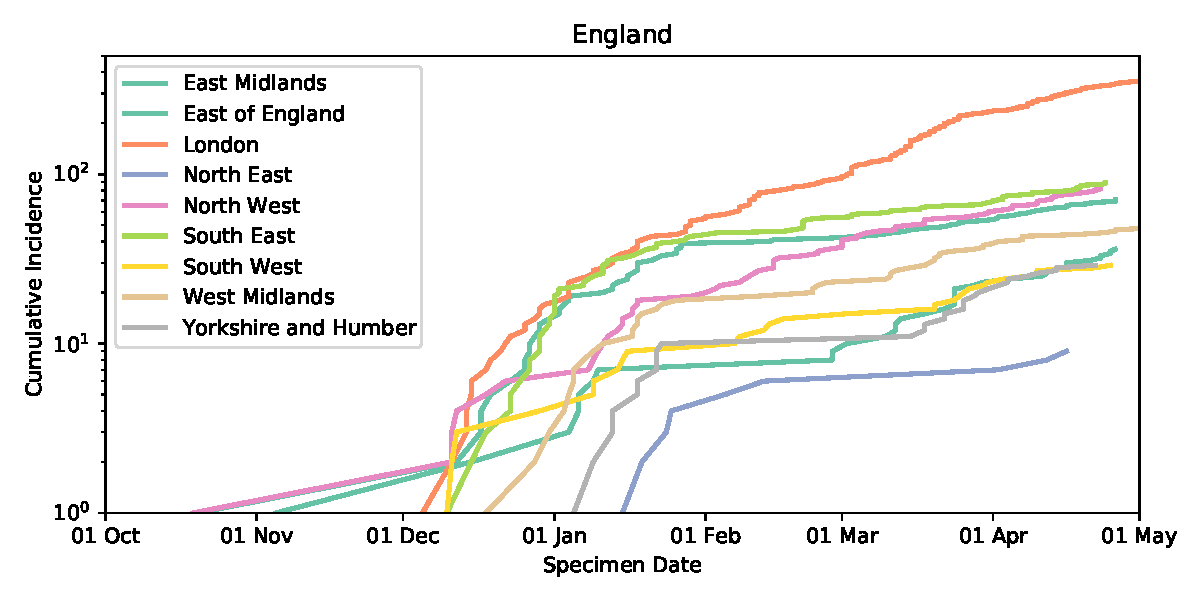
\includegraphics[width=1.0\textwidth]{../figures/voc_region_log.pdf}\\
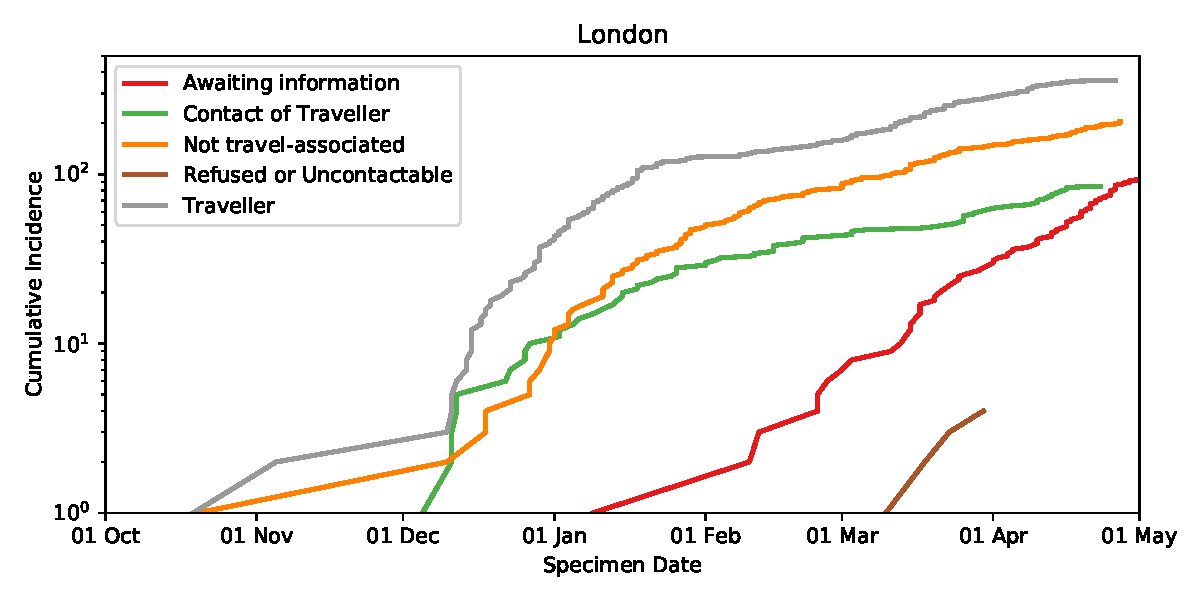
\includegraphics[width=1.0\textwidth]{../figures/voc_london_log.pdf}\\
\caption{Time series of B.1.351}
\label{fig:voc_log}
\end{figure}

\clearpage

\begin{figure}
\centering
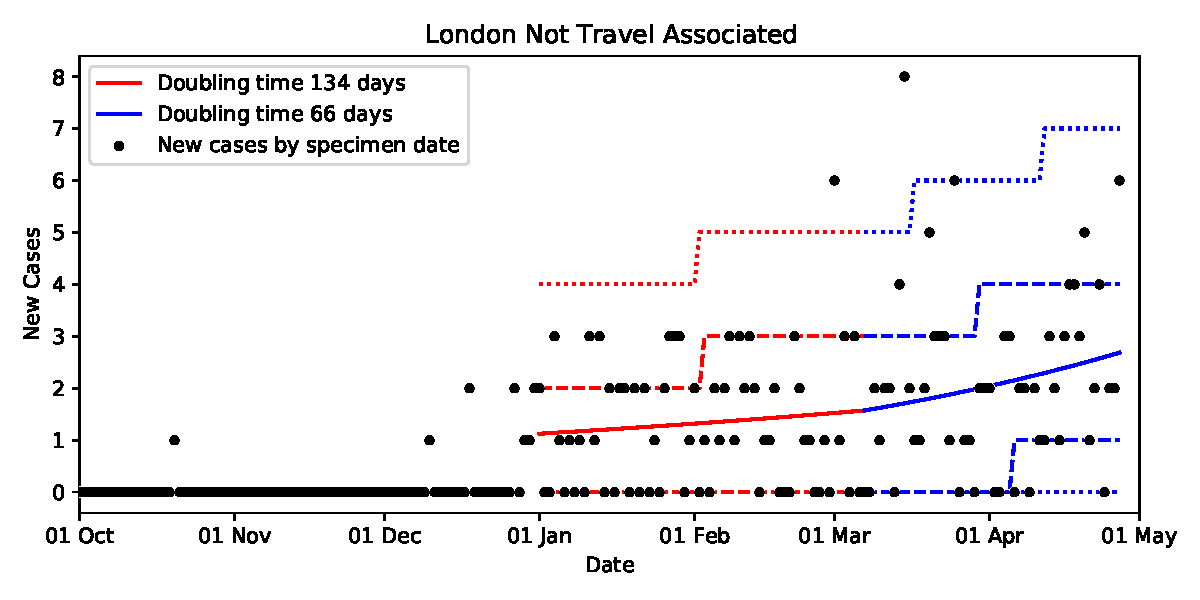
\includegraphics[width=1.0\textwidth]{../figures/voc_london_nta_fit.pdf}\\
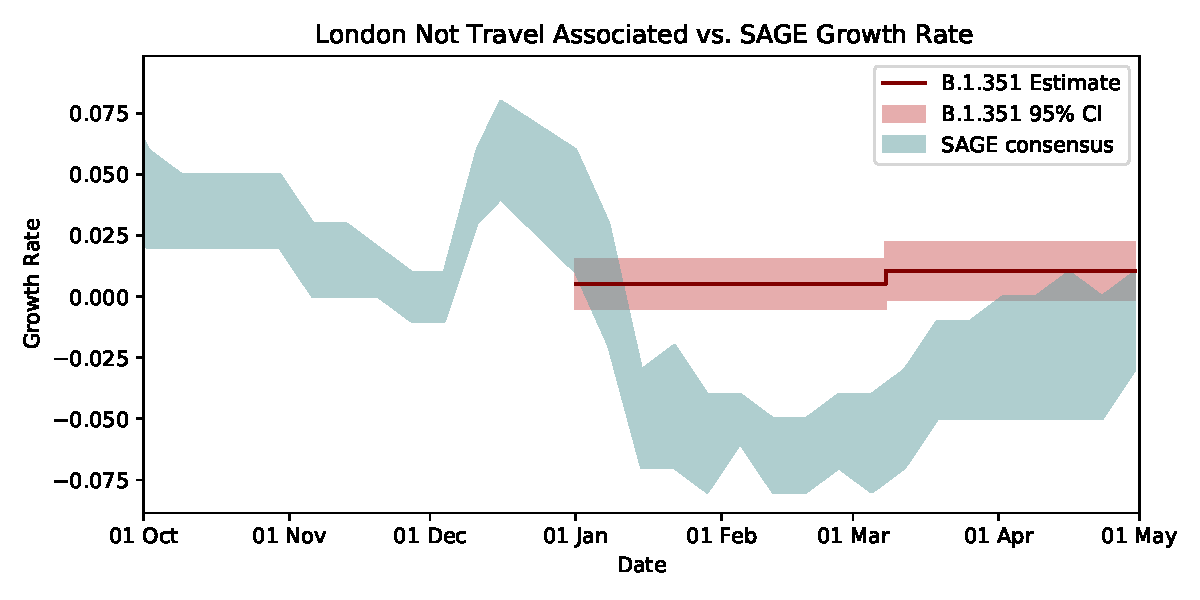
\includegraphics[width=1.0\textwidth]{../figures/voc_london_nta_comp.pdf}\\
\caption{Fit of B.1.351 Growth versus }
\label{fig:voc_fit}
\end{figure}

\end{document}



